\documentclass[../norme-di-progetto.tex]{subfiles}
\begin{document}

%%%%%%%%%%%%%%%%%%%%%%%%%%%%
%%% 3.1 - DOCUMENTAZIONE %%%
%%%%%%%%%%%%%%%%%%%%%%%%%%%%
\subsection{Documentazione}
\subsubsection{Scopo}
Lo scopo di questo processo è quello di fornire i dettagli e le regole su cui deve essere basata la redazione e la manutenzione di tutta la documentazione durante l'intero ciclo di vita del software.

\subsubsection{Aspettative}
Le aspettative della corretta implementazione di questo processo sono:
\begin{itemize}
  \item L'identificazione di regole su cui deve essere basata la corretta stesura dei documenti;
  \item L'individuazione di una struttura rigorosa sulla quale basare la redazione dei documenti durante tutti i processi di sviluppo.
\end{itemize}

\subsubsection{Descrizione}
Questa sezione descrive i dettagli su come deve essere redatta e verificata la documentazione. Al fine di ottenere l'uniformità e il rigore espositivo di tutti i documenti prodotti durante il ciclo di vita del software, ogni documento deve basarsi sulle regole descritte in questa sede.

\subsubsection{Procedure}
\paragraph{Ciclo di vita dei documenti}
Il documento viene innanzitutto creato; a tale scopo, il gruppo ha deciso di creare un template \LaTeX sul quale basare la stesura di ogni documento. Questo assicura l'uniformità della struttura dei documenti, facilitando inoltre il versionamento. \\
Dopo la creazione, il ciclo di vita dei documenti è suddiviso in tre differenti attività:
\begin{itemize}
  \item \textbf{Stesura del documento}: la stesura del documento consiste nella scrittura del documento stesso. Questa attività viene svolta da un redattore, assegnato dal Responsabile di progetto; dopo la stesura, il Responsabile autorizzerà all'avanzamento della stesura, rimanendo in attesa dell'esito della revisione;
  \item \textbf{Revisione}: dopo la stesura, il documento verrà revisionato dai Verificatori, che ne controlleranno l'aderenza alle norme di progetto e la correttezza sintattica e semantica. Dopo questo controllo, a seconda che l'esito sia positivo o negativo, lo comunicheranno al Responsabile, che farà avanzare il documento all'approvazione finale, o ai Redattori, che correggeranno eventuali segnalazioni e lo riproporranno ai Verificatori;
  \item \textbf{Approvazione finale}: con l'approvazione ricevuta da parte dei Verificatori, il Responsabile di progetto confermerà quindi il documento, eseguendone il rilascio.
\end{itemize}

\paragraph{Struttura dei documenti}
Al fine di organizzare coerentemente e uniformamente la struttura dei documenti, si è deciso di utilizzare il \textit{package} \textbf{subfiles} di \LaTeX. La repository contiene una \textit{directory} denominata \texttt{commons/} contenente:
\begin{itemize}
  \item Il file \texttt{config.tex}, contenente le definizioni dei comandi \LaTeX;
  \item Il file \texttt{template.tex}, contenente il \textit{template} su cui si basano tutti i documenti;
  \item La cartella \texttt{img/}, contenente le immagini comuni a tutti i documenti.
\end{itemize}
Per ogni documento è quindi presente una \textit{directory} contenente:
\begin{itemize}
  \item  Il file principale, chiamato con il nome del documento, in formato \texttt{.tex};
  \item La cartella \texttt{components/}, contenente gli altri file in formato \texttt{.tex} che vengono inclusi nel file principale ed eventuali allegati interni al documento.
\end{itemize}
Basandosi su un \textit{template}, ogni documento ha quindi una struttura fissa e predeterminata.

\subparagraph{Frontespizio}
Il frontespizio fornisce tutti i dati principali del documento. Esso presenta il logo del gruppo, centrato, seguito dal nome del gruppo e dal titolo del progetto; sotto di questo è presente il titolo del documento. \\
Sono fornite anche altre informazioni essenziali, le quali sono:
\begin{itemize}
  \item \textbf{Versione}: versione attuale del documento;
  \item \textbf{Approvazione}: stato di approvazione del documento, che può essere "In redazione" o recare il nome del responsabile che ha approvato il documento;
  \item \textbf{Redazione}: redattori del documento;
  \item \textbf{Verifica}: verificatori del documento;
  \item \textbf{Uso}: destinazione del documento, che può essere "Interno" o "Esterno";
  \item \textbf{Destinato a}: destinazione specifica del documento.
\end{itemize}
\subparagraph{Registro delle modifiche}
Nella seconda pagina di ogni documento è presente il registro delle modifiche del documento, consistente in una tabella contentente, per ogni modifica:
\begin{itemize}
  \item \textbf{Versione}: versione del documento aggiornata alla modifica effettuata;
  \item \textbf{Nominativo}: nome dell'autore della modifica;
  \item \textbf{Ruolo}: ruolo dell'autore della modifica;
  \item \textbf{Data}: data in cui è stata effettuata la modifica;
  \item \textbf{Descrizione}: descrizione della modifica effettuata.
\end{itemize}
\subparagraph{Indice}
L'indice riepiloga la struttura del documento. Ha una struttura standard: la numerazione ha struttura \begin{center}
  \centering
  \textbf{a.b.c.d.e}
\end{center} dove:
\begin{itemize}
  \item \textbf{a} è il capitolo principale;
  \item \textbf{b} è la sezione del capitolo;
  \item \textbf{c} è la sottosezione della sezione;
  \item \textbf{d} è il paragrafo della sezione;
  \item \textbf{e} è il sottoparagrafo del paragrafo.
\end{itemize}
La massima profondità della numerazione è quindi 5; nel caso in cui si rendesse necessario aggiungere un livello, questo verrà indicato come sottoparagrafo del sottoparagrafo senza ulteriore numerazione.

\subparagraph{Elenco delle figure}
L'elenco delle figure consiste nell'indice di tutte le figure presenti nel documento, eccezion fatta per il logo del gruppo che non viene riportato. L'elenco riporta il numero della figura, il nome descrittivo e la pagina in cui si trova.

\subparagraph{Elenco delle tabelle}
L'elenco delle tabelle indicizza tutte le tabelle presenti nel documento, esclusa quella del Registro delle modifiche. L'elenco riporta il numero della tabella, il nome  descrittivo e la pagina in cui si trova.

\subparagraph{Contenuto principale}
Ogni pagina del contenuto principale del documento è composta da:
\begin{itemize}
  \item Il logo del gruppo, posizionato in alto a sinistra;
  \item Il nome del gruppo, posizionato in alto a destra;
  \item Il nome del documento, posizionato in alto a destra sotto al nome del gruppo;
  \item Una riga orizzontale, posizionata in alto e che attraversa tutta la pagina, che divide logo, nome del gruppo e nome del documento dal contenuto della pagina;
  \item Il numero di pagina, posizionato in basso a destra e nel formato \\ \begin{center}
    \centering
    \textbf{N di T}
  \end{center} dove
\begin{itemize}
  \item \textbf{N} è il numero della pagina corrente;
  \item \textbf{T} è il numero di pagine totali.
\end{itemize}
Il conteggio delle pagine inizia dalla prima pagina dopo l'Elenco delle tabelle.
\end{itemize}
Nello spazio compreso tra la riga orizzontale e il numero di pagina si articola il contenuto proprio della pagina.

\paragraph{Classi di documenti}
I documenti prodotti appartengono a diverse categorie, secondo le quali sono classificati.

\subparagraph{Documenti ufficiali}
I documenti ufficiali sono quelli che seguono la struttura elencata in questo documento, e che sono stati verificati e approvati dal responsabile di progetto. Essi possono essere Interni o Esterni, a seconda della destinazione che hanno.

\subparagraph{Glossario}
In accompagnamento ai documenti ufficiali viene fornito un Glossario, contenente tutti i termini caratterizzati da sottolineatura e una G maiuscola come pedice. Il Glossario ha la funzione di chiarire possibili fraintendimenti provenienti dall'utilizzo di determinati termini. \\
Perché un termine venga incluso nel Glossario deve soddisfare almeno uno tra i seguenti requisiti:
\begin{itemize}
  \item Essere un termine tecnico. Rientrano in questo criterio i nomi propri delle tecnologie utilizzate, i termini tecnici propri di queste e i termini frequentemente utilizzati nell'Ingegneria del Software;
  \item Essere presente in tutti i documenti;
  \item Avere più di un significato plausibile nel contesto in cui viene utilizzato;
  \item Essere un acronimo specifico e raramente usato.
\end{itemize}
Il Glossario possiede un'impostazione grafica identica agli altri documenti, con l'eccezione di non possedere numerazione nell'indice. I termini sono ordinati in ordine alfabetico, e divisi in base alla prima lettera; ogni lettera deve avere la sua sezione, anche nel caso in cui nessun termine vi appartenga. \\
I termini appartenenti al Glossario sono contrassegnati come tali solo una volta per ogni documento, nello specifico la prima volta che il termine compare in esso, al fine di evitare l'appesantimento visivo.

\subparagraph{Verbali}
I verbali documentano gli argomenti discussi in una riunione; essi possono essere interni, e quindi riferirsi a una riunione tra soli membri del gruppo, o eserni, e quindi riferirsi a una riunione a cui partecipa anche l'azienda. La struttura del documento è identica a quella dei documenti ufficiali; ogni verbale è composto dai seguenti componenti:
\begin{itemize}
  \item \textbf{Informazioni generali}: informazioni dell'incontro, consistenti nella modalità, nella data e negli orari di inizio e fine, e i partecipanti all'incontro;
  \item \textbf{Ordine del giorno}: lista degli argomenti e dei temi di cui il gruppo ha deciso di discutere durante l'incontro;
  \item \textbf{Resoconto}: riassunto di quanto detto durante l'incontro punto per punto.
\end{itemize}

\subparagraph{Lettere}
Le lettere, tra cui quella di presentazione, seguono il formato classico di una lettera: esse includono quindi uno o più mittenti e uno o più destinatari, il logo e il nome del gruppo. \\
La lettera di presentazione contiene anche l'elenco dei documenti rilasciati e il preventivo per lo svolgimento del progetto.

\paragraph{Norme tipografiche}
\subparagraph{Nomi dei file}
La nomenclatura di tutti i file segue la convenzione \textit{kebab case}, nota anche come \textit{lisp-case}. Le regole di questa convenzione sono le seguenti:
\begin{itemize}
  \item Ogni file inizia con una lettera minuscola;
  \item Tra ogni parola viene inserito come separatore il tratto d'unione \textbf{-};
  \item In caso di presenza di apostrofo, esso verrà sostituito dal tratto d'unione;
  \item Le lettere accentate sono abolite, sostituite dalla semplice lettera senza accento.
\end{itemize}
L'unica eccezione che è stata adottata è l'utilizzo del segno di interpunzione "trattino basso" \textbf{\_} tra il nome del documento e la data di redazione nei nomi dei verbali e tra la data e la versione. \\
Tutti i nomi di file avranno quindi il seguente formato: \\ \begin{center}
  \centering
  \textbf{N-a-b-c[\_YYYY-MM-DD]\_vX.Y.Z.ext}
\end{center} dove:
\begin{itemize}
  \item \textbf{N} è il numero di verbale nel caso in cui il documento sia un verbale; opzionalmente, può essere utilizzato per numerare ordinatamente i \textit{subfiles} di un determinato documento;
  \item Le parentesi quadre \textbf{[ ]} si applicano solo al caso dei verbali;
  \item \textbf{a}, \textbf{b} e \textbf{c} sono parole singole. Il numero di parole singole non è limitato a tre ma si può aumentare o diminuire. Nel caso specifico dei verbali, la forma di questa porzione di nome è \begin{center}
    \centering
    \textbf{verbale-[interno/esterno]}
  \end{center};
  \item \textbf{vX.Y.Z} indicano la versione attuale del documento;
  \item \textbf{ext} è l'estensione del file.
\end{itemize}
Alcuni esempi di nomi di files legittimi sono quindi:
\begin{itemize}
  \item \texttt{1-verbale-interno\_2020\_01\_13\_v1.0.0.tex};
  \item \texttt{norme-di-progetto.tex}, con annessi \textit{subfiles}:
    \begin{itemize}
      \item \texttt{1-introduzione.tex};
      \item \texttt{2-processi-primari.tex};
      \item \texttt{3-processi-supporto.tex};
      \item \texttt{4-processi-organizzativi.tex}.
    \end{itemize}
\end{itemize}

\subparagraph{Stile del testo}
Ogni diversa formattazione usata all'interno dei documenti ha un significato preciso, e ogni documento deve obbligatoriamente seguire questo stile. Gli stili sono:
\begin{itemize}
  \item Utilizzo di testo in corsivo per i termini in lingua diversa da quella italiana;
  \item Utilizzo di testo in caratteri dattilografici per i nomi di file e delle \textit{directories}; queste ultime devono finire con il carattere barra \textbf{/};
  \item Utilizzo di testo in grassetto per i termini conseguentemente definiti e per i titoli dei sottoparagrafi di sottoparagrafi;
  \item Utilizzo di testo sottolineato, in aggiunta al pedice G maiusola, per i termini appartenenti al Glossario;
  \item Utilizzo di testo maiuscoletto per i nomi dei documenti all'interno dei documenti stessi.
\end{itemize}

\subparagraph{Figure}
L'utilizzo di figure all'interno dei documenti è permesso; le immagini devono essere centrate nella pagina, avere larghezza o lunghezza fissa di 10cm ed essere seguite dalla seguente dicitura: \\ \begin{center}
  \centering
  \textbf{Figura N: D}
\end{center} dove:
\begin{itemize}
  \item \textbf{N} è il numero progressivo della figura all'interno del documento in cui è inserita;
  \item \textbf{D} è una breve descrizione dell'immagine.
\end{itemize}
Il logo del gruppo non segue queste regole, poiché non possiede né numero progressivo né descrizione.

\subparagraph{Diagrammi UML}
Tutti i diagrammi \glossario{UML} sono inseriti nei documenti come figure, e come tali figurano nell'Elenco delle Figure.

\subparagraph{Tabelle}
Le tabelle devono essere centrate nella pagina, ed essere seguite dalla seguente dicitura: \\ \begin{center}
  \centering
  \textbf{Tabella N: D}
\end{center} dove:
\begin{itemize}
  \item \textbf{N} è il numero progressivo della tabella all'interno del documento in cui è inserita;
  \item \textbf{T} è il titolo della tabella.
\end{itemize}
La tabella del Registro delle modifiche non segue queste regole, poiché non possiede né numero progressivo né titolo.

\subparagraph{Formati comuni}
I formati di data, ora e versione sono determinati e univoci per ogni documento. Nello specifico:
\begin{itemize}
  \item La data segue lo standard ISO 8601, e quindi è nel formato \\ \begin{center}
    \centering
    \textbf{YYYY-MM-DD}
  \end{center} dove:
  \begin{itemize}
    \item \textbf{YYYY} è l'anno, scritto per intero;
    \item \textbf{MM} è il mese, scritto per intero;
    \item \textbf{DD} è il giorno, scritto per intero
  \end{itemize};
  \item L'ora è nel formato \\ \begin{center}
  \centering
  \textbf{HH:MM}
  \end{center} dove:
  \begin{itemize}
    \item \textbf{HH} è l'ora in formato 24 ore;
    \item \textbf{MM} sono i minuti.
  \end{itemize}
\end{itemize}
\subparagraph{Sigle}
All'interno della documentazione possono essere utilizzate delle sigle. Esse sono:
\begin{itemize}
  \item \textbf{Sigle dei documenti}:
  \begin{itemize}
    \item \textbf{NP}: Norme di Progetto;
    \item \textbf{SF}: Studio di Fattibilità;
    \item \textbf{AR}: Analisi dei Requisiti;
    \item \textbf{PP}: Piano di Progetto;
    \item \textbf{PQ}: Piano di Qualifica;
    \item \textbf{Gl}: Glossario;
    \item \textbf{MU}: Manuale Utente.
  \end{itemize}
  \item \textbf{Fasi del progetto}:
  \begin{itemize}
  \item \textbf{RR}: Revisione dei Requisiti;
  \item \textbf{RP}: Revisione di Progettazione;
  \item \textbf{RQ}: Revisione di Qualifica;
  \item \textbf{RA}: Revisione di Accettazione.
  \end{itemize}
  \item \textbf{Ruoli}:
  \begin{itemize}
  \item \textbf{RdP}: Responsabile di Progetto;
  \item \textbf{AdP}: Amministratore di Progetto;
  \item \textbf{An}: Analista;
  \item \textbf{Pr}: Progettista;
  \item \textbf{Pg}: Programmatore;
  \item \textbf{Ve}: Verificatore.
  \end{itemize}
  \item \textbf{Altre sigle:}
  \begin{itemize}
    \item \textbf{SVM}: \glossario{Support Vector Machines};
    \item \textbf{RL}: \glossario{Regressione Lineare};
    \item \textbf{ML}: \glossario{Machine Learning};
    \item \textbf{JS}: \glossario{Javascript};
    \item \textbf{CLI}: \glossario{Command Line};
    \item \textbf{IDE}: \glossario{Integrated Developement Environment};
    \item \textbf{ITS}: \glossario{Issue Tracking System}.
    %%% AGGIUNGERE QUI SIGLE %%%
  \end{itemize}
\end{itemize}

\subparagraph{Altre norme tipografiche}
\subparagraph*{Elenchi}
Gli elenchi presenti nella documentazione sono unicamente di tipo puntato, indicati cioè con un cerchietto pieno, o con un trattino (lo stesso carattere del tratto d'unione) nel caso in cui si tratti di un sotto-elenco di un elenco puntato. \\
Ogni parola appartenente a un elenco puntato deve iniziare con la lettera maiuscola; ogni elemento di un elenco puntato deve finire con un punto e virgola, ad eccezione dell'ultimo che deve finire con un punto.
%%% AGGIUNGERE QUI EVENTUALI ALTRE NORME TIPOGRAFICHE, OGNUNA CON UN subparagraph*

%%%%%%%%%%%%%%%%%%%%%%%%%%%%%%%%%%%%%%%%%%%
%%% 3.2 - GESTIONE DELLA CONFIGURAZIONE %%%
%%%%%%%%%%%%%%%%%%%%%%%%%%%%%%%%%%%%%%%%%%%
\subsection{Gestione della configurazione}
\subsubsection{Scopo}
Lo scopo di questo processo è delineare le norme utili a predisporre il Workspace comune per il gruppo; esso definisce anzitutto tutto ciò che concerne il versionamento, comprese la memorizzazione e la manutenzione di quanto prodotto. Descrive inoltre la gestione delle attività che devono essere svolte durante il ciclo di vita del prodotto.

\subsubsection{Versionamento}
Ogni documento deve essere versionato, al fine di avere una cronologia delle modifiche e dell'importanza di queste sul contenuto del documento; fanno eccezione a questa regola i verbali, i quali per definizione non hanno bisogno di essere modificati dopo la stesura e la verifica, ma vanno direttamente approvati. Ad ogni versione del documento corrisponde una riga nel Registro delle modifiche. \\
Ogni versione viene espressa nel seguente modo: \\ \begin{center}
  \centering
  \textbf{vX.Y.Z}
\end{center} dove:
\begin{itemize}
  \item \textbf{X}: indica una versione stabile del documento. L'incremento della cifra segue queste regole:
  \begin{itemize}
    \item Inizia da 0;
    \item Viene incrementata dal Responsabile solo dopo l'approvazione del documento da parte sua;
    \item La cifra massima coincide con il numero di Revisioni.
  \end{itemize}
  \item \textbf{Y}: indica una versione del documento ancora in fase di redazione ma comunque abbastanza stabile per poter essere verificato. L'incremento della cifra segue queste regole:
  \begin{itemize}
    \item Inizia da 0 ad ogni incremento di X;
    \item Viene incrementata dal Verificatore in seguito alla verifica;
    \item Non ha cifra massima.
  \end{itemize}
  \item \textbf{Z}: indica una versione del documento ancora in fase di lavorazione da parte dei redattori e che, per scarsa quantità di modifiche, non necessita ancora di verifica. L'incremento della cifra segue queste regole:
  \begin{itemize}
    \item Inizia da 0 ad ogni incremento di Y;
    \item Viene incrementata dal redattore del documento a ogni modifica, seppur minima;
    \item Non ha cifra massima.
  \end{itemize}
\end{itemize}

\subsubsection{Repository}
Una \textit{repository} è un ambiente in cui vengono memorizzati, mantenuti e versionati i file di un progetto software, durante il suo intero ciclo di vita. Il sistema di controllo che il gruppo utilizza è \glossario{Git}, e i file dell'intero progetto sono ospitati dalla piattaforma Github; viene inoltre utilizzato Git Commitizen per facilitare il controllo di quanto aggiunto o modificato di volta in volta sulla \textit{repository}.

\paragraph{Struttura della repository e workflow}
La struttura adottata sfrutta il meccanismo di \textit{branching} offerto dallo strumento Git; questo permette lo sviluppo parallelo di più funzionalità e il lavoro in parallelo sulla stessa \textit{repository}. \\
La \textit{repository} utilizzata si suddivide nei seguenti \textit{branch}:
\begin{itemize}
  \item \texttt{master}: branch principale, sul quale vengono fatti le \glossario{major releases};
  \item \texttt{norme-di-progetto}: branch secondario nel quale viene sviluppato l'intero documento riguardante le Norme di Progetto;
  \item \texttt{analisi-dei-requisiti}: branch secondario nel quale viene sviluppato l'intero documento riguardante l'Analisi dei Requisiti;
  \item \texttt{glossario}: branch secondario nel quale viene sviluppato l'intero documento Glossario;
  \item \texttt{piano-di-progetto}: branch secondario nel quale viene sviluppato l'intero documento riguardante il Piano di Progetto;
  \item \texttt{piano-di-qualifica}: branch secondario nel quale viene sviluppato l'intero documento riguardante il Piano di Qualifica;
  \item \texttt{studio-di-fattibilita}: branch secondario nel quale viene sviluppato l'intero documento riguardante lo Studio di Fattibilità;
  \item \texttt{verbali}:: branch secondario nel quale vengono sviluppati i verbali interni ed esterni.
\end{itemize}
Il workflow adottato è basato quindi su un principio della separazione dei documenti: questo, unito ai sistemi anti-collisione di git, permette che durante il periodo in cui un membro del gruppo è assegnato a un ruolo di redazione specifico, egli sia l'unico a lavorare su tale documento.

\subparagraph{Struttura dei branch}
Ogni branch è costituito da file, cartelle e sotto-cartelle.
\subparagraph*{File}
I file presenti in ogni branch hanno tipo fisso e predefinito; essi sono:
\begin{itemize}
  \item File di configurazione di Github:
  \begin{itemize}
    \item \texttt{.gitignore}: contiene la lista di file e directory spuri che possono essere presenti nelle \textit{repository} locali ma non nella \textit{repository} remota;
    \item File \texttt{.yml}: contengono le istruzioni per l'esecuzione delle Github Actions;
    \item \texttt{README.md}: file markdown contenente una breve descrizione della \textit{repository}.
  \end{itemize}
  \item File di configurazione di Git Commitizen:
  \begin{itemize}
    \item \texttt{.czcr}: contiene le impostazioni, definite dal gruppo, di Git Commitizen.
  \end{itemize}
  \item File di configurazione di \glossario{Visual Studio Code}
  \begin{itemize}
    \item \texttt{.editorconfig}: contiene le impostazioni, definite dal gruppo, del Workspace di Visual Studio Code;
    \item \texttt{settings.json}: contiene le impostazioni specifiche, definite dal gruppo, dell'editor Visual Studio Code;
    \item \texttt{extensions.json}: contiene le estenzioni, consigliate per lo sviluppo del progetto, da includere in Visual Studio Code.
  \end{itemize}
  \item File di documentazione:
  \begin{itemize}
    \item File \texttt{.tex}: file \LaTeX contenenti il codice sorgente per la generazione dei documenti;
    \item File \texttt{.png}: immagini che vengono incluse nei documenti.
  \end{itemize}
\end{itemize}

\subparagraph*{Cartelle}
Ogni branch presenta un insieme di cartelle predefinito:
\begin{itemize}
\item \texttt{.github/}: contiene i file propri di Github, tra cui i file \texttt{.yml} delle Github Actions;
  \item \texttt{.vscode/}: contiene i file di configurazione di Visual Studio Code;
  \item \texttt{commons/}: contiene i file template di \LaTeX;
  \item \texttt{interni/}: contiene i documenti ad uso interno. In ogni branch questa cartella contiene una sottocartella con lo stesso nome del branch, contenente i file sorgente \LaTeX dello specifico documento;
  \item \texttt{esterni/}: contiene i documenti ad uso esterno. In ogni branch questa cartella contiene una sottocartella con lo stesso nome del branch, contenente i file sorgente \LaTeX dello specifico documento;
\end{itemize}

\paragraph{Strumenti}
Le attività di gestione della configurazione sono coadiuvate dall'utilizzo di strumenti software, che permettono il perseguimento del giusto workflow e l'applicazione delle norme.
\subparagraph{Git}
La repository è ospitata dal servizio di \glossario{hosting} Github; per operare sulla repository vengono utilizzati tre strumenti:
\begin{itemize}
  \item Portale Github.com;
  \item Git Commitizen;
  \item Visual Studio Code.
\end{itemize}
\subparagraph*{Portale Github.com}
Il portale Github.com permette la consultazione immediata di quanto fatto e pubblicato, e la gestione delle Issues e delle Milestones.
\begin{figure}[H]
  \centering
  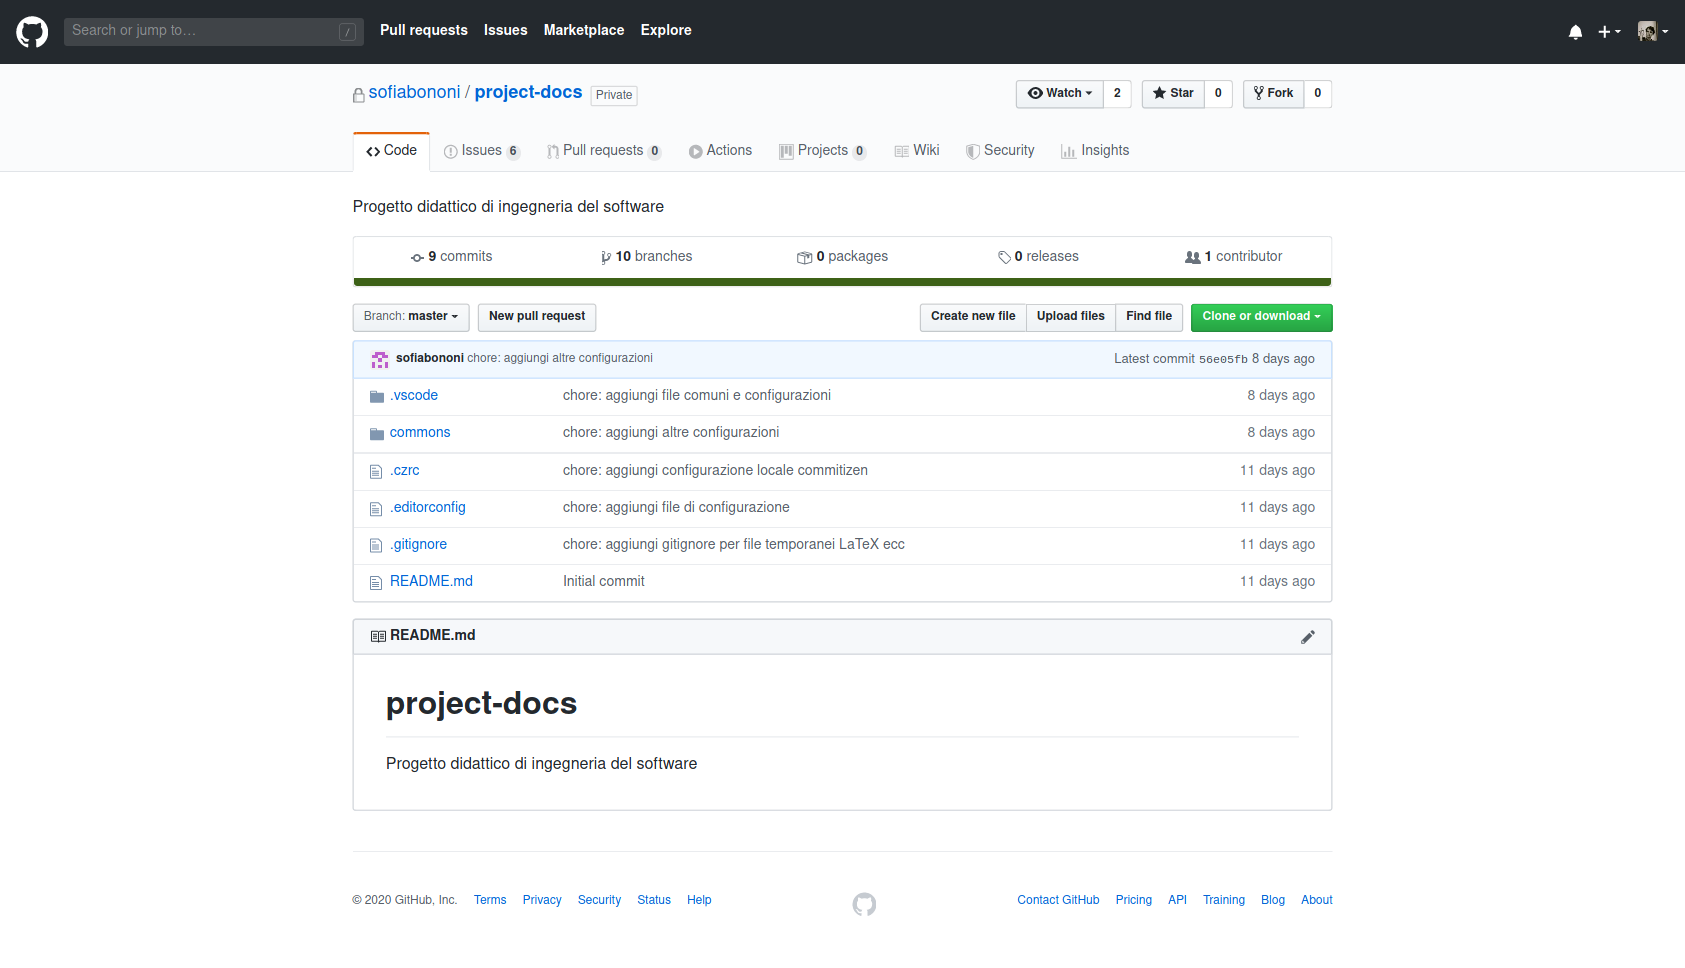
\includegraphics[width=10cm]{img/github.png}
  \label{fig:github}
  \caption{Portale in Github della repository di progetto.}
\end{figure}

\subparagraph*{Git Commitizen}
Per il \glossario{commit} delle modifiche ai file della repository viene utilizzato Git Commitizen tramite \glossario{Command Line}. Questo assicura l'uniformità dei commit e quindi una maggiore chiarezza di quanto viene versionato.

\subparagraph*{Visual Studio Code}
Visual Studio Code è l'IDE che viene uniformemente usato da ogni componente del gruppo. Questo strumento software permette l'estensione delle funzionalità attraverso l'installazione di componenti aggiuntivi. Tra questi, due in particolare permettono di operare sulla repository:
\begin{itemize}
  \item \textbf{Git Graph}: visualizzazione del grafo della repository e possibilità di svolgere azioni Git direttamente su di esso;
  \item \textbf{GitHub Pull Requests}: strumento di revisione delle Pull Requests di Github.
\end{itemize}

%%%%%%%%%%%%%%%%%%%%%%%%%%%%%%%%%%%%
%%% 3.3 - GESTIONE DELLA QUALITÀ %%% - %%% NECESSARIO PdQ %%%
%%%%%%%%%%%%%%%%%%%%%%%%%%%%%%%%%%%%
\subsection{Gestione della qualità}
\subsubsection{Scopo}
Lo scopo di questo processo è quello di garantire che i prodotti software e i processi del ciclo di vita siano conformi ai requisiti concordati con il cliente, e che rispettino gli obiettivi di qualità.
\subsubsection{Aspettative}
Le aspettative di questo processo sono le seguenti:
\begin{itemize}
  \item Ottenere qualità nell'organizzazione;
  \item Sviluppare un prodotto software di qualità, comprendente anche una documentazione completa e di facile fruizione;
%%% DA AMPLIARE CON PdQ %%%
\end{itemize}
\subsubsection{Descrizione} %%% NECESSARIO PdQ
\subsubsection{Attività}
\subsubsection{Strumenti}

%%%%%%%%%%%%%%%%%%%%%%
%%% 3.4 - VERIFICA %%%
%%%%%%%%%%%%%%%%%%%%%%
\subsection{Verifica}

\subsubsection{Scopo}
Lo scopo di questo processo è quello di verificare che il prodotto venga realizzato nel modo corretto, secondo delle regole stabilite. \\
Il processo di verifica interessa sia il software che la documentazione prodotta, assicurando che il prodotto finale sia corretto e completo.

\subsubsection{Aspettative}
La procedura che tale processo, al fine di essere implementato correttamente, deve rispettare, è la seguente:
\begin{itemize}
  \item Vengono definiti dei chiari criteri di accettazione;
  \item Vengono definite delle attività di verifica, con relativa documentazione;
  \item Vengono eseguiti dei test di verifica, ed eventuali difetti vengono catalogati;
  \item Eventuali difetti vengono corretti.
\end{itemize}

\subsubsection{Descrizione}
Il processo di verifica inizia con un prodotto del quale è necessario controllare la conformità alle aspettative e finisce con un prodotto che le soddisfa. Una volta verificato, il prodotto passerà alla fase di validazione.

\subsubsection{Attività}
Le attività di questo processo sono di due tipologie:
\begin{itemize}
  \item Analisi;
  \item Test.
\end{itemize}
\paragraph{Analisi}
L'attività di analisi si divide in due sottocategorie:
\begin{itemize}
  \item Analisi Statica;
  \item Analisi Dinamica.
\end{itemize}
\subparagraph{Analisi Statica}
L'analisi statica è l'attività di analisi che viene eseguita sul prodotto senza il bisogno che questo venga eseguito. Essa valuta la presenza o assenza di errori e/o difetti, la conformità alle regole definite e la coesione dei componenti. \\
L'analisi statica si divide in due tipologie:
\begin{itemize}
  \item \textbf{Walkthrough}: i componenti del gruppo analizzano il prodotto nella sua interezza alla ricerca di difetti e di inconformità con le regole prescritte. Questa tecnica verrà utilizzata più intensamente durante l'inizio del progetto, per lasciare il tempo ai vari componenti di familizzare con le norme prescritte. Durante questa attività viene stipulata una lista di controllo contenente gli errori trovati;
  \item \textbf{Inspection}: questa tipologia di analisi statica viene eseguita dal singolo Verificatore, che provvederà a ricercare gli errori segnalati nella lista di controllo all'interno di quanto prodotto; è quindi un'analisi più precisa e mirata agli errori che vengono più comunemente commessi.
\end{itemize}
Segue la lista di controllo parziale, contenente gli errori più comuni finora trovati. Questa lista verrà possibilmente ampliata al progredire degli eventuali errori trovati.

\begin{table}[H]
\centering
\begin{tabular}{p{5cm}p{10cm}}
\textbf{Oggetto}           & \textbf{Controllo da effettuare}      \\
Data e ora                              & Verificare il giusto formato: deve essere coerente con lo standard ISO 8601 \\
Sintassi                          & Verificare che le frasi non siano eccessivamente verbose o sintatticamente errate       \\
Uniformità nell'utilizzo dei termini & Controllare che i termini ambigui vengano usati uniformemente (\underline{e.g.} \textit{obiettivo}-\textit{obbiettivo}) \\
Nidificazione sezioni            & Verificare che non vi siano incongruenze nella nidificazione delle varie sezioni, cioè: \begin{itemize}
  \item Le sezioni, capitoli, paragrafi e sottoparagrafi abbiano numerazione non crescente;
  \item Non venga utilizzato il giusto ordine di indentazione.
\end{itemize}       \\
Elenchi                           & \begin{itemize}
  \item Verificare che la prima lettera di ogni elemento sia maiuscola;
  \item Verificare che ogni elemento finisca con la corretta punteggiatura (; o .).
\end{itemize}       \\
\end{tabular}
\caption{Errori frequenti nella documentazione.}
\end{table}

\subparagraph{Analisi Dinamica}
L'analisi dinamica è la tipologia di analisi che viene eseguita sul prodotto eseguendolo. Essa viene effettuata tramite dei test, che controllano il corretto funzionamento del prodotto.

\paragraph{Test} %%% NECESSARIO PdQ %%%
\subsubsection{Strumenti}

%%%%%%%%%%%%%%%%%%%%%%%%%
%%% 3.5 - VALIDAZIONE %%%
%%%%%%%%%%%%%%%%%%%%%%%%%
\subsection{Validazione}
\subsubsection{Scopo}
Lo scopo di questo processo è determinare se il prodotto soddisfa i requisiti concordati con il proponente e l'utilizzo specifico per cui è stato creato. Il processo di validazione esegue quindi il test completo sul sistema, assicurando infine che le necessità del cliente siano state pienamente soddisfatte. \\ Il processo di validazione viene effettuato dopo il processo di verifica, per avere la certezza che tutte le componenti del sistema possano essere verificate.
\subsubsection{Attività}
Il processo di validazione consiste delle seguenti attività:
\begin{itemize}
  \item Individuare una strategia di validazione, comprendente:
  \begin{itemize}
    \item L'identificazione degli oggetti da validare;
    \item L'identificazione delle attività di valutazione da applicare.
  \end{itemize}
  \item Eseguire la strategia, ovverosia svolgere la validazione;
  \item Valutare i risultati ottenuti dalla strategia:
  \begin{itemize}
    \item Se i risultati sono positivi vengono consegnati al proponente;
    \item Se lo svoglimento dell'attività presenta problemi o inconformità con le richieste del cliente, questi devono essere risolti e, successivamente, i risultati devono essere consegnati al proponente.
  \end{itemize}
\end{itemize}
%%% QUESTA SEZIONE È COMPLETA MA SI PUÒ ESPANDERE %%%
\end{document}
